\documentclass{beamer}
\usetheme{Boadilla}

% importations
\usepackage[french]{babel} % pour dire que le texte est en francais
\usepackage{csquotes}
\usepackage[T1]{fontenc} % pour les font postscript
\usepackage[cyr]{aeguill} % Police vectorielle TrueType, guillemets francais
\usepackage{epsfig} % pour gérer les images
\usepackage{amsmath,amsthm, stmaryrd} % très bon mode mathématique
\usepackage{amsfonts,amssymb,bm, bbold}% permet la definition des ensembles
\usepackage{algorithm2e} % pour les algorithmes
\usepackage{algpseudocode} % pour les algorithmes
\usepackage{graphicx}
\usepackage{float} % pour le placement des figure
\usepackage{url} % pour une gestion efficace des url
\usepackage{hyperref}  % pour les hyperliens dans le document
\usepackage{tikz} % For graph plots
\usepackage{adjustbox} % To resize tikzpictures
\usepackage{fontawesome5}
\usepackage{makecell}

% Beamer
\setbeamertemplate{headline}{%
    \begin{beamercolorbox}[ht=2.25ex,dp=3.75ex]{section in head/foot}
        \insertnavigation{\paperwidth}
    \end{beamercolorbox}%
}%
\beamertemplatenavigationsymbolsempty % Pas de bar de navigation
\setbeamerfont{caption}{size=\scriptsize} % Petit titre de figures

% bibliographie
\usepackage[style=apa,sorting=none]{biblatex}
\addbibresource{references.bib}


% Tikz
%% Tikz Related
\usetikzlibrary{calc,shapes,backgrounds,arrows,automata,shadows,positioning}
\usetikzlibrary{arrows,shapes,positioning,shadows,trees,calc,backgrounds,automata,positioning}
\usetikzlibrary{decorations.pathreplacing,calligraphy}



\tikzset{
    basic/.style  = {draw, text width=3cm, font=\sffamily, rectangle},
    root/.style   = {basic, rounded corners=2pt, thin, align=center,
            fill=green!30},
    level 2/.style = {basic, rounded corners=6pt, thin,align=center, fill=green!60,
            text width=8em},
    level 3/.style = {basic, thin, align=left, fill=pink!60, text width=3.5cm}
}
% Couleurs
% pour tickz multilevel
\definecolor{redorg}{RGB}{215,48,39}
\definecolor{orangeorg}{RGB}{253,174,97}

\definecolor{blueind}{RGB}{69,117,233}
\definecolor{cyanind}{RGB}{116,173,209}
\definecolor{electricblue}{RGB}{125, 249, 255}

\definecolor{greenind}{RGB}{112,130,56}

\definecolor{burntorange}{RGB}{204, 85, 0}
\definecolor{goldenyellow}{RGB}{255, 192, 0}
\definecolor{peach}{RGB}{255,255,0}

\definecolor{gray}{RGB}{128,128,128}

% Footnote
\makeatletter
\newcommand\blfootnote[1]{%
  \begingroup
  \renewcommand{\@makefntext}[1]{\noindent\makebox[1.8em][r]#1}
  \renewcommand\thefootnote{}\footnote{#1}%
  \addtocounter{footnote}{-1}%
  \endgroup
}
\makeatother


\subtitle{Séminaire des stagiaires}
\title[Collections de réseaux bipartites]{Détection de structure dans des réseaux bipartites}
\author[L. Lacoste]{Louis \textsc{Lacoste}} % Sous la supervision de Pierre
\date{29 juin 2023}

\begin{document}

% titre
\begin{frame}[noframenumbering,plain]
    \maketitle
\end{frame}

\section{Contexte du modèle}
\label{sec:contexte-du-modele}
\begin{frame}
    \frametitle{Contexte écologique}
    \begin{itemize}
        \item Faire de la détection de structure sur un réseau (SBM, LBM) mais intérêt à le faire sur plusieurs
        \item De nombreux réseaux disponibles \parencite{WebLifeEcological} et décrivant des interactions similaires
        \item Re-grouper les réseaux selon leur similarité (\emph{clustering} de réseaux)
        \item Transférer de l'information grâce à la collection (par exemple reconstitution de données manquantes)
        \item Déterminer des structures d'interactions fines de manière agnostique % Pas d'idee preco
              %\item Vérifier si le regroupement est lié à des co-variables
    \end{itemize}
\end{frame}
\begin{frame}
    \frametitle{Réseaux bipartites\footnote{Ou \emph{bipartis}. Voir~\cite{larousseDefinitionsBipartiBipartite}.}}
    \begin{columns}[c]
        \begin{column}{0.48\textwidth}
            \centering
            Réseau bipartite\\
            \begin{tikzpicture}[scale=.6]
                \tikzstyle{every edge}=[-,>=stealth',shorten >=1pt,auto,draw,line width=1.5pt]
                \tikzstyle{every state}=[draw, text=black,scale=0.95, transform shape]
                \tikzstyle{every state}=[draw=none,text=black,scale=0.75, transform shape]
                \tikzstyle{every node}=[fill=blueind]

                \node[state, draw=black!50] (A1) at (0,5) {\textbf{R1}};
                \node[state, draw=black!50] (A2) at (2.5,5) {\textbf{R2}};
                \node[state, draw=black!50] (A3) at (5,5) {\textbf{R3}};

                \tikzstyle{every node}=[fill=greenind, shape=rectangle]
                \tikzstyle{every state}=[draw=none,text=black,scale=0.75, transform shape, shape=rectangle]
                \node[state, draw=black!50] (B1) at (0,0) {\textbf{C1}};
                \node[state, draw=black!50] (B2) at (1.25,0) {\textbf{C2}};
                \node[state, draw=black!50] (B3) at (2.5,0) {\textbf{C3}};
                \node[state, draw=black!50] (B4) at (3.75,0) {\textbf{C4}};
                \node[state, draw=black!50] (B5) at (5,0) {\textbf{C5}};
                \path (A1) edge [] (B1);
                \path (A1) edge  (B2);
                \path (A1) edge  (B3);
                \path (A1) edge  (B4);
                \path (A2) edge  (B3);
                \path (A2) edge  (B4);
                \path (A3) edge  (B5);
                \path (A2) edge  (B5);
            \end{tikzpicture}
        \end{column}
        \hfill
        \begin{column}{0.48\linewidth}
            Matrice d'incidence
            \smallskip
            $X=\left(
                \begin{array}{rrrrr}
                        1 & 1 & 1 & 1 & 0 \\
                        0 & 0 & 1 & 1 & 1 \\
                        0 & 0 & 0 & 0 & 1 \\
                    \end{array}\right)
            $\\
        \end{column}
    \end{columns}
    \smallskip
    Permet de décrire des interactions impliquant deux agents dont les rôles
    sont de natures différentes.\\
    Par exemple : hôtes-parasites, plantes-pollinisateurs, graines-disperseurs \dots
\end{frame}
\begin{frame}
    \frametitle{Latent Block Model (LBM\footnotemark[2])}
    %DONE remplacer i \in bullet par Zi = \bullet
    Proposé par~\cite{govaertEMAlgorithmBlock2005}.
    \begin{columns}
        \begin{column}{0.40\linewidth}
            \begin{figure}[H]
                \center
                \begin{tikzpicture}[scale=0.35]
                    \tikzstyle{every state}=[draw, text=black,scale=0.95, transform shape]
                    \tikzstyle{every state}=[draw=none,text=black,scale=0.75, transform shape]
                    \tikzset{edge_proba/.style={draw=white, fill=none, text=black}}

                    \tikzstyle{every node}=[fill=blueind]
                    \node[edge_proba] (pi1) at (1,5.7) {\textbf{$\pi_{{\color{blueind}\bullet}}$}};
                    \node[state, draw=black!50] (R11) at (0,5) {\textbf{R11}};
                    \node[state, draw=black!50] (R12) at (1,5) {\textbf{R12}};
                    \node[state, draw=black!50] (R13) at (2,5) {\textbf{R13}};

                    \tikzstyle{every node}=[fill=cyanind]
                    \node[edge_proba] (pi2) at (6.75,5.7) {\textbf{$\pi_{{\color{cyanind}\bullet}}$}};
                    \node[state, draw=black!50] (R21) at (6.25,5) {\textbf{R21}};
                    \node[state, draw=black!50] (R22) at (7.25,5) {\textbf{R22}};

                    \tikzstyle{every node}=[fill=electricblue]
                    \node[edge_proba] (pi3) at (10,5.7) {\textbf{$\pi_{{\color{electricblue}\bullet}}$}};
                    \node[state, draw=black!50] (R31) at (10,5) {\textbf{R31}};

                    \tikzstyle{every node}=[fill=burntorange, shape=rectangle]
                    \node[edge_proba] (pi3) at (0.5,-0.7) {\textbf{$\rho_{{\color{burntorange}\bullet}}$}};
                    \tikzstyle{every state}=[draw=none,text=black,scale=0.75, transform shape, shape=rectangle]
                    \node[state, draw=black!50] (B1) at (0,0) {\textbf{C11}};
                    \node[state, draw=black!50] (B2) at (1,0) {\textbf{C12}};
                    \tikzstyle{every node}=[fill=goldenyellow, shape=rectangle]
                    \node[edge_proba] (pi3) at (4,-0.7) {\textbf{$\rho_{{\color{goldenyellow}\bullet}}$}};
                    \node[state, draw=black!50] (B3) at (3.5,0) {\textbf{C21}};
                    \node[state, draw=black!50] (B4) at (4.5,0) {\textbf{C22}};
                    \tikzstyle{every node}=[fill=peach, shape=rectangle]
                    \node[edge_proba] (pi3) at (10,-0.7) {\textbf{$\rho_{{\color{peach}\bullet}}$}};
                    \node[state, draw=black!50] (B5) at (10,0) {\textbf{C31}};

                    \tikzstyle{every edge}=[-,>=stealth',shorten >=1pt,auto,draw,line width=1.5pt,draw opacity=0.2]

                    \path (R11) edge[-,>=stealth',shorten >=1pt,auto,draw=gray,line width=1.5pt, fill=gray, opacity=1] node[left, fill=none] {$\alpha_{{\color{blueind}\bullet}{\color{burntorange}\bullet}}$} (B1);
                    \path (R11) edge (B2);
                    \path (R11) edge  (B3);
                    \path (R11) edge  (B4);

                    \path (R12) edge [] (B1);
                    \path (R12) edge  (B2);
                    \path (R12) edge  (B3);
                    \path (R12) edge  (B4);

                    \path (R13) edge [] (B1);
                    \path (R13) edge  (B2);
                    \path (R13) edge  (B3);
                    \path (R13) edge[-,>=stealth',shorten >=1pt,auto,draw=gray,line width=1.5pt, fill=gray, opacity=1] node[midway, left, fill=none] {$\alpha_{{\color{blueind}\bullet}{\color{goldenyellow}\bullet}}$} (B4);

                    \path (R21) edge[-,>=stealth',shorten >=1pt,auto,draw=gray,line width=1.5pt, fill=gray, opacity=1] node[midway, right, fill=none] {$\alpha_{{\color{cyanind}\bullet}{\color{goldenyellow}\bullet}}$} (B3);
                    \path (R21) edge  (B4);
                    \path (R21) edge  (B5);

                    \path (R22) edge  (B3);
                    \path (R22) edge  (B4);
                    \path (R22) edge[-,>=stealth',shorten >=1pt,auto,draw=gray,line width=1.5pt, fill=gray, opacity=1] node[midway, left, fill=none] {$\alpha_{{\color{cyanind}\bullet}{\color{peach}\bullet}}$} (B5);

                    \path (R31) edge[-,>=stealth',shorten >=1pt,auto,draw=gray,line width=1.5pt, fill=gray, opacity=1] node[midway, right, fill=none] {$\alpha_{{\color{electricblue}\bullet}{\color{peach}\bullet}}$} (B5);

                \end{tikzpicture}
                \caption{Exemple de LBM\footnotemark}
                \label{fig:LBMvisu}
            \end{figure}
        \end{column}
        \begin{column}{0.51\linewidth}
            Pour \begin{itemize}
                \item $Q_1 = |\{{\color{blueind}\bullet},{\color{cyanind}\bullet},{\color{electricblue}\bullet}\}|$ blocs fixés en ligne
                \item $Q_2 = |\{{\color{burntorange}\bullet},{\color{goldenyellow}\bullet},{\color{peach}\bullet}\}|$ blocs fixés en colonne
            \end{itemize}
            \begin{block}{Paramètres}
                \begin{itemize}
                    \item $\pi_{\bullet} = \mathbb{P}(Z_i = \bullet)$ en ligne et $\rho_{\bullet} = \mathbb{P}(W_j = \bullet)$ en colonne
                    \item $\alpha_{{\color{blueind}\bullet}{\color{burntorange}\bullet}} = \mathbb{P}(X_{ij} = 1 | Z_i = {\color{blueind}\bullet}, W_j = {\color{burntorange}\bullet})$
                \end{itemize}
            \end{block}
        \end{column}
    \end{columns}

    \footnotetext{Que j'appellerai par la suite BiSBM}

\end{frame}
\begin{frame}
    \frametitle{\emph{colSBM}}
    Le modèle \emph{colSBM} \parencite{chabert-liddellLearningCommonStructures2023}.\\
    % Difficulté estimer les parametres

    % DONE Modifier les realisations pour variabilite, mettre iid au dessus du sim et inverser modele et realisations
    \smallskip
    \definecolor{yellow}{RGB}{255,190,60}
    \begin{center}
        \begin{adjustbox}{trim=0 0 0 1cm}
            \begin{tikzpicture}[scale=.32]
                \tikzstyle{every edge}=[-,>=stealth',shorten >=1pt,auto,draw,line width=.5pt, bend left]
                \tikzstyle{every state}=[draw, text=black,scale=0.95, transform shape]
                \tikzset{edge_proba/.style={draw=white, fill=none, text=black}}

                \tikzstyle{every node}=[fill=yellow]
                \node[state, draw=black!50] (A1) at (0,2) {\textbf{A1}};
                \node[state, draw=black!50] (A2) at (1.5, 2) {\textbf{A2}};
                \node[state, draw=black!50] (A3) at (0.75,3.25) {\textbf{A3}};

                \tikzstyle{every node}=[fill=blueind]
                \node[state, draw=black!50] (B1) at (4.5,3) {\textbf{B1}};
                \node[state, draw=black!50] (B2) at (4,4.75) {\textbf{B2}};
                \node[state, draw=black!50] (B3) at (5.5,6) {\textbf{B3}};
                \node[state, draw=black!50] (B4) at (7,4.75) {\textbf{B4}};
                \node[state, draw=black!50] (B5) at (6.5,3) {\textbf{B5}};

                \tikzstyle{every node}=[fill=greenind]
                \node[state, draw=black!50] (C1) at (5,0) {\textbf{C1}};
                \node[state, draw=black!50] (C2) at (7,1) {\textbf{C2}};


                \path (A1) edge[bend right] (A2);
                \path (A1) edge node[midway, left, fill=none] {$\alpha_{{\color{yellow}\bullet}{\color{yellow}\bullet}}$} (A3);
                \path (A3) edge (A2);

                \path (A3) edge node[midway, above, fill=none] {$\alpha_{{\color{yellow}\bullet}{\color{blueind}\bullet}}$} (B3);

                \path (B1) edge (B2);
                \path (B2) edge (B3);
                \path (B3) edge (B4);
                \path (B4) edge (B5);
                \path (B5) edge (B1);

                \path (B1) edge[bend left=0] (B4);
                \path (B5) edge[bend left=0] (B2);

                \path (A2) edge[bend right] node[midway, below, fill=none] {$\alpha_{{\color{yellow}\bullet}{\color{greenind}\bullet}}$} (C1);
                \path (C1) edge[bend right] node[midway, below, fill=none] {$\alpha_{{\color{greenind}\bullet}{\color{greenind}\bullet}}$} (C2);
                \path (C2) edge[bend right] node[midway, right, fill=none] {$\alpha_{{\color{greenind}\bullet}{\color{blueind}\bullet}}$} (B4);

                \node[font=\small, text justified,draw=none, fill=none] at (4.5,-1.5) {SBM};



                % Sampled network
                \begin{scope}[xshift=-16cm,yshift=4cm]
                    \node[font=\small, text justified, fill=none] at (10, -2.5) {$\overset{iid}{\sim}$};
                    \tikzstyle{every node}=[fill=gray, scale=0.95]
                    \tikzstyle{every edge}=[-,>=stealth',shorten >=1pt,auto,draw,line width=.5pt, bend left]
                    \tikzstyle{every state}=[draw, text=black,scale=0.95, transform shape]

                    \node[state, draw=black!50] (A1) at (0,0) {\textbf{10}};
                    \node[state, draw=black!50] (A2) at (1, 0) {\textbf{2}};
                    \node[state, draw=black!50] (A3) at (0.5,1) {\textbf{5}};

                    \node[state, draw=black!50] (B2) at (2,2.75) {\textbf{9}};
                    \node[state, draw=black!50] (B3) at (3.5,4) {\textbf{6}};
                    \node[state, draw=black!50] (B4) at (5,2.75) {\textbf{3}};
                    \node[state, draw=black!50] (B5) at (4.5,1) {\textbf{7}};

                    \node[state, draw=black!50] (C1) at (3,-0.5) {\textbf{4}};

                    \path (A1) edge[bend right] (A2);
                    \path (A1) edge (A3);
                    \path (A3) edge (A2);

                    \path (A3) edge (B3);

                    \path (B2) edge (B3);
                    \path (B3) edge (B4);
                    \path (B4) edge (B5);

                    \path (B5) edge[bend left=0] (B2);

                    \path (A2) edge[bend right] (C1);

                    \node[text width=3cm,font=\small, text justified, rotate=90, fill=none, below = -0.8cm of C1] (dots) {\dots};

                \end{scope}
                \begin{scope}[xshift=-16cm,yshift=-4cm]
                    \tikzstyle{every node}=[fill=gray, scale=0.95]
                    \tikzstyle{every edge}=[-,>=stealth',shorten >=1pt,auto,draw,line width=.5pt, bend left]
                    \tikzstyle{every state}=[draw, text=black,scale=0.95, transform shape]

                    \node[state, draw=black!50] (A2) at (1, 0) {\textbf{2}};
                    \node[state, draw=black!50] (A3) at (0.5,1) {\textbf{1}};

                    \node[state, draw=black!50] (B1) at (2.5,1) {\textbf{5}};
                    \node[state, draw=black!50] (B2) at (2,2.75) {\textbf{10}};
                    \node[state, draw=black!50] (B4) at (5,2.75) {\textbf{8}};
                    \node[state, draw=black!50] (B5) at (4.5,1) {\textbf{7}};

                    \node[state, draw=black!50] (C2) at (5,0) {\textbf{3}};



                    \path (A3) edge (A2);


                    \path (B1) edge (B2);
                    \path (B4) edge (B5);
                    \path (B5) edge (B1);

                    \path (B1) edge[bend left=0] (B4);
                    \path (B5) edge[bend left=0] (B2);

                    \path (C2) edge[bend right] (B4);
                \end{scope}
            \end{tikzpicture}
        \end{adjustbox}
    \end{center}
    Pour $Q = |\{{\color{yellow}\bullet},{\color{blueind}\bullet},{\color{greenind}\bullet}\}|$ blocs fixés :
    \begin{block}{Paramètres}
        \begin{itemize}
            \item $\pi_{\bullet} = \mathbb{P}(Z_i =\bullet)$
            \item $\alpha_{{\color{greenind}\bullet}{\color{blueind}\bullet}} = \mathbb{P}(X_{ij} = 1  | Z_i = {\color{greenind}\bullet}, Z_j = {\color{blueind}\bullet})$
        \end{itemize}
    \end{block}
\end{frame}
\section{Extension de \emph{colSBM} aux réseaux bipartites}
\label{sec:extension-de-colsbm-aux-reseaux-bipartites}
\begin{frame}
    \frametitle{Collections bipartites}
    \begin{center}
        \begin{adjustbox}{trim=0 0 1 1.5cm}
            \begin{tikzpicture}[scale=.33]
                \begin{scope}[xshift=18cm, yshift=2cm]
                    \tikzstyle{every state}=[draw=none, text=black,scale=0.75, transform shape]
                    \tikzset{edge_proba/.style={draw=white, fill=none, text=black}}

                    \tikzstyle{every node}=[fill=blueind]
                    \node[edge_proba] (pi1) at (1,5.7) {\textbf{$\pi_{{\color{blueind}\bullet}}$}};
                    \node[state, draw=black!50] (R11) at (0,5) {\textbf{R11}};
                    \node[state, draw=black!50] (R12) at (1,5) {\textbf{R12}};
                    \node[state, draw=black!50] (R13) at (2,5) {\textbf{R13}};

                    \tikzstyle{every node}=[fill=cyanind]
                    \node[edge_proba] (pi2) at (6.75,5.7) {\textbf{$\pi_{{\color{cyanind}\bullet}}$}};
                    \node[state, draw=black!50] (R21) at (6.25,5) {\textbf{R21}};
                    \node[state, draw=black!50] (R22) at (7.25,5) {\textbf{R22}};

                    \tikzstyle{every node}=[fill=electricblue]
                    \node[edge_proba] (pi3) at (10,5.7) {\textbf{$\pi_{{\color{electricblue}\bullet}}$}};
                    \node[state, draw=black!50] (R31) at (10,5) {\textbf{R31}};

                    \tikzstyle{every node}=[fill=burntorange, shape=rectangle]
                    \node[edge_proba] (rho1) at (0.5,-1) {\textbf{$\rho_{{\color{burntorange}\bullet}}$}};
                    \tikzstyle{every state}=[draw=none,text=black,scale=0.75, transform shape, shape=rectangle]
                    \node[state, draw=black!50] (B1) at (0,0) {\textbf{C11}};
                    \node[state, draw=black!50] (B2) at (1,0) {\textbf{C12}};
                    \tikzstyle{every node}=[fill=goldenyellow, shape=rectangle]
                    \node[edge_proba] (rho2) at (4,-1) {\textbf{$\rho_{{\color{goldenyellow}\bullet}}$}};
                    \node[state, draw=black!50] (B3) at (3.5,0) {\textbf{C21}};
                    \node[state, draw=black!50] (B4) at (4.5,0) {\textbf{C22}};
                    \tikzstyle{every node}=[fill=peach, shape=rectangle]
                    \node[edge_proba] (rho3) at (10,-1) {\textbf{$\rho_{{\color{peach}\bullet}}$}};
                    \node[state, draw=black!50] (B5) at (10,0) {\textbf{C31}};

                    \node[font=\small, text justified,draw=none, fill=none, below = 0.05cm of rho2] {BiSBM};

                    \tikzstyle{every edge}=[-,>=stealth',shorten >=1pt,auto,draw,line width=1.5pt,draw opacity=0.2]

                    \path (R11) edge (B2);
                    \path (R11) edge  (B3);
                    \path (R11) edge  (B4);

                    \path (R12) edge [] (B1);
                    \path (R12) edge  (B2);
                    \path (R12) edge  (B3);
                    \path (R12) edge  (B4);

                    \path (R13) edge [] (B1);
                    \path (R13) edge  (B2);
                    \path (R13) edge  (B3);

                    \path (R21) edge  (B4);
                    \path (R21) edge  (B5);

                    \path (R22) edge  (B3);
                    \path (R22) edge  (B4);

                    \path (R11) edge[-,>=stealth',shorten >=1pt,auto,draw=gray,line width=1.5pt, fill=gray, opacity=1] node[left, fill=none] {$\alpha_{{\color{blueind}\bullet}{\color{burntorange}\bullet}}$} (B1);
                    \path (R13) edge[-,>=stealth',shorten >=1pt,auto,draw=gray,line width=1.5pt, fill=gray, opacity=1] node[midway, left, fill=none] {$\alpha_{{\color{blueind}\bullet}{\color{goldenyellow}\bullet}}$} (B4);
                    \path (R21) edge[-,>=stealth',shorten >=1pt,auto,draw=gray,line width=1.5pt, fill=gray, opacity=1] node[midway, anchor=center, fill=none] {$\alpha_{{\color{cyanind}\bullet}{\color{goldenyellow}\bullet}}$} (B3);
                    \path (R22) edge[-,>=stealth',shorten >=1pt,auto,draw=gray,line width=1.5pt, fill=gray, opacity=1] node[midway, left, fill=none] {$\alpha_{{\color{cyanind}\bullet}{\color{peach}\bullet}}$} (B5);
                    \path (R31) edge[-,>=stealth',shorten >=1pt,auto,draw=gray,line width=1.5pt, fill=gray, opacity=1] node[midway, right, fill=none] {$\alpha_{{\color{electricblue}\bullet}{\color{peach}\bullet}}$} (B5);
                \end{scope}

                \begin{scope}[xshift=3cm, yshift = 1cm]
                    \node[text justified, fill=none] at (10, 3.5) {$\overset{iid}{\sim}$};
                    \begin{scope}[yshift = 6cm]
                        \tikzstyle{every state}=[draw, text=black,scale=0.75, transform shape]

                        \tikzstyle{every node}=[fill=gray]
                        \node[state, draw=black!50] (R11) at (0,1.25) {\textbf{1}};
                        \node[state, draw=black!50] (R12) at (1,1.25) {\textbf{2}};
                        \node[state, draw=black!50] (R13) at (2,1.25) {\textbf{3}};
                        \node[state, draw=black!50] (R21) at (3,1.25) {\textbf{4}};
                        \node[state, draw=black!50] (R31) at (5,1.25) {\textbf{6}};

                        \tikzstyle{every state}=[draw=none,text=black,scale=0.75, transform shape, shape=rectangle]
                        \node[state, draw=black!50] (B1) at (0.5,-1) {\textbf{1}};

                        \node[state, draw=black!50] (B31) at (2.5,-1) {\textbf{3}};
                        \node[state, draw=black!50] (B4) at (3.5,-1) {\textbf{4}};

                        \node[state, draw=black!50] (B5) at (4.5,-1) {\textbf{5}};

                        \tikzstyle{every edge}=[-,>=stealth',shorten >=1pt,auto,draw,line width=1pt, draw=gray, fill=gray]
                        \path (R11) edge (B1);
                        \path (R11) edge  (B31);
                        \path (R11) edge  (B4);

                        \path (R12) edge [] (B1);
                        \path (R12) edge  (B31);
                        \path (R12) edge  (B4);

                        \path (R13) edge [] (B1);
                        \path (R13) edge  (B31);
                        \path (R13) edge (B4);

                        \path (R21) edge (B31);
                        \path (R21) edge  (B4);
                        \path (R21) edge  (B5);


                        \path (R31) edge (B5);
                    \end{scope}
                    \node[text width=3cm,font=\small, text justified, rotate=90, fill=none] (dots) at (2.5, 7.5){\dots};

                    \begin{scope}[yshift = 0cm]
                        \tikzstyle{every state}=[draw, text=black,scale=0.75, transform shape]

                        \tikzstyle{every node}=[fill=gray]
                        \node[state, draw=black!50] (R11) at (0,2.25) {\textbf{4}};
                        \node[state, draw=black!50] (R13) at (2,2.25) {\textbf{6}};
                        \node[state, draw=black!50] (R21) at (3,2.25) {\textbf{3}};
                        \node[state, draw=black!50] (R22) at (4,2.25) {\textbf{5}};
                        \node[state, draw=black!50] (R31) at (5,2.25) {\textbf{2}};

                        \tikzstyle{every state}=[draw=none,text=black,scale=0.75, transform shape, shape=rectangle]
                        \node[state, draw=black!50] (B1) at (0.5,0) {\textbf{5}};
                        \node[state, draw=black!50] (B2) at (1.5,0) {\textbf{1}};

                        \node[state, draw=black!50] (B4) at (3.5,0) {\textbf{2}};

                        \node[state, draw=black!50] (B5) at (4.5,0) {\textbf{4}};

                        \tikzstyle{every edge}=[-,>=stealth',shorten >=1pt,auto,draw,line width=1pt, draw=gray, fill=gray]
                        \path (R11) edge (B1);
                        \path (R11) edge (B2);
                        \path (R11) edge  (B4);

                        \path (R13) edge [] (B1);
                        \path (R13) edge  (B2);
                        \path (R13) edge (B4);

                        \path (R21) edge  (B4);
                        \path (R21) edge  (B5);

                        \path (R22) edge  (B4);
                        \path (R22) edge (B5);

                        \path (R31) edge (B5);
                    \end{scope}
                \end{scope}
            \end{tikzpicture}
        \end{adjustbox}
    \end{center}

    Pour
    \begin{itemize}
        \item $Q_1 = |\{{\color{blueind}\bullet},{\color{cyanind}\bullet},{\color{electricblue}\bullet}\}|$ blocs fixés en ligne
        \item $Q_2 = |\{{\color{burntorange}\bullet},{\color{goldenyellow}\bullet},{\color{peach}\bullet}\}|$ blocs fixés en colonne
    \end{itemize}
    \begin{block}{Paramètres}
        \begin{itemize}
            \item $\pi_{\bullet} = \mathbb{P}(Z_i =\bullet)$ en ligne et $\rho_{\bullet} = \mathbb{P}(W_j = \bullet)$ en colonne
            \item $\alpha_{{\color{blueind}\bullet}{\color{burntorange}\bullet}} = \mathbb{P}(X_{ij} = 1  | Z_i = {\color{blueind}\bullet}, W_j = {\color{burntorange}\bullet})$
        \end{itemize}
    \end{block}
\end{frame}

\begin{frame}
    \frametitle{Différents modèles}
    \begin{block}{\emph{iid-colBiSBM}}
        $\bm{\pi} = (\pi_1, \dots \pi_{Q_1})$ et $\bm{\rho} = (\rho_1, \dots \rho_{Q_2})$ %{$\forall q \in \llbracket 1, Q_1 - 1\rrbracket, \pi_q > 0$ et $\forall r \in \llbracket 1, Q_2 - 1\rrbracket, \rho_r > 0$}
        , tous les réseaux partagent les mêmes paramètres\footnotemark
    \end{block}

    \begin{block}{\emph{$\pi\rho$-colBiSBM}}
        $\bm{\pi} = ((\pi_{\color{black}1}^{\color{red}m}, \dots \pi_{\color{black}Q_1}^{\color{red}m}))_{m=1,\dots M}$ et $\bm{\rho} = ((\rho_{\color{black}1}^{\color{red}m}, \dots \rho_{\color{black}Q_2}^{\color{red}m}))_{m=1,\dots M}$ %{$\forall q \in \llbracket 1, Q_1 - 1\rrbracket, \pi_q > 0$ et $\forall r \in \llbracket 1, Q_2 - 1\rrbracket, \rho_r > 0$}
        \small \\
        avec $\forall q,m \in \llbracket 1, Q_1 \rrbracket \times \llbracket 1, M \rrbracket, \pi_q^m \in \left[ 0,1 \right]$
        et $\forall r,m \in \llbracket 1, Q_2 \rrbracket \times \llbracket 1, M \rrbracket, \rho_r^m \in \left[ 0,1 \right]$
    \end{block}
    Et également deux autres modèles ($\pi$-colBiSBM et $\rho$-colBiSBM) où seulement une des deux dimensions est libre.
    \footnotetext{Dans tous les modèles la structure de connectivité est supposée identique au sein de la collection.}
\end{frame}
\begin{frame}
    \frametitle{Estimation des paramètres}
    % DONE dire que tau i q m c' est la proba que Zim = q, approximation de la proba variationnelle. Parce qu on impose lindependance
    Maximisation d'une borne inférieure de la log-vraisemblance des données observées.
    \begin{multline*}
        \ell (\bm{X};\bm{\theta}) \geq \color{red}\sum_{m=1}^{M} \bigg( \color{black} \sum_{i = 1}^{n_1^m}\sum_{j=1}^{n_2^m}\sum_{q \in \mathcal{Q}_{1,m}} \sum_{r \in \mathcal{Q}_{2,m}} \tau^{1,m}_{i,q} \tau^{2,m}_{j,r} \log f(X^{m}_{ij}; \alpha_{qr}) \\
        + \sum_{i=1}^{n_1^m} \sum_{q \in \mathcal{Q}_{1,m}} \tau^{1,m}_{i,q} \log \pi_{\color{black}q}^{\color{gray}m} + \sum_{j=1}^{n_2^m} \sum_{r \in \mathcal{Q}_{2,m}} \tau^{2,m}_{j,r} \log \rho_{\color{black}r}^{\color{gray}m} \\
        - \sum_{i=1}^{n_1} \tau^{1,m}_{i,q} \log \tau^{1,m}_{i,q} - \sum_{j=1}^{n_2} \tau^{2,m}_{j,r} \log \tau^{2,m}_{j,r} \color{red}\bigg) \color{black} =: J(\bm{\tau};\bm{\theta}) $$
    \end{multline*}

    \begin{block}{Approximation variationnelle}
        $\tau_{i,q}^{1,m} = P(Z_i = q | X^m_{ij})$ et $\tau_{j,r}^{2,m} = P(W_j = r | X^m_{ij})$ tels que $P(Z_i = q, W_j = r | X^m_{ij}) = \tau_{i,q}^{1,m}\times\tau_{j,r}^{2,m}$
    \end{block}

\end{frame}

\begin{frame}
    \frametitle{Sélection de modèle : choix de $(Q_1,Q_2)$ - Approche gloutonne}
    % DONE But maximiser un critere le BICL, deplacer voir St Clair dans la note
    % VEM a Q1 Q2 fixer
    % Choix de Q1 Q2 par maximisation du BICL
    % Itemize dans la box : init, explo voisin, arrets
    \underline{Le VEM se fait à $Q_1, Q_2$ fixés}, il faut donc déterminer les \enquote*{meilleures} coordonnées.
    Nous maximisons un BIC-L\footnote{\emph{Bayesian Information Criterion - Like}, en adaptant les formules de~\cite{chabert-liddellLearningCommonStructures2023}}.

    Détermination d'un premier mode par approche \emph{gloutonne} \smallskip
    \begin{columns}
        \begin{column}{0.5\linewidth}
            \begin{tikzpicture}
                \draw[step=1cm, help lines] (-2,-2) grid (2,2);
                \draw[fill=gray, draw=gray] (0,0) circle [radius=0.225cm];
                \draw[fill=blueind, draw=blueind] (1,0) circle [radius=0.225cm];
                \draw[fill=blueind, draw=blueind] (0,1) circle [radius=0.225cm];
                \draw[fill=red, draw=red] (-1,0) circle [radius=0.225cm];
                \draw[fill=red, draw=red] (0,-1) circle [radius=0.225cm];

                % Légende
                \node[font=\tiny, text justified,fill=none, rotate=-45] (Splits) at (0.5,0.5){{\color{blueind} Splits}};
                \node[font=\tiny, text justified,fill=none, rotate=-45] (Merges) at (-0.5,-0.5){{\color{red} Merges}};

                % Splitting
                \draw[>=stealth,->,thick, draw=blueind] (0.225,0) -- +(0.55,0);
                \draw[>=stealth,->,thick, draw=blueind] (0,0.225) -- +(0,0.55);

                % Merging
                \draw[>=stealth,->,thick, draw=red] (-0.225,0) -- +(-0.55,0);
                \draw[>=stealth,->,thick, draw=red] (0,-0.225) -- +(0,-0.55);

                % Axes
                \draw[>=to,->,thick] (-2,-2) -- +(1,0);
                \node[font=\small, fill=none] (Q_1) at (-0.75,-2) {$Q_1$};
                \draw[>=to,->,thick] (-2,-2) -- +(0,1);
                \node[font=\small, fill=none] (Q_2) at (-2,-0.75) {$Q_2$};

            \end{tikzpicture}
        \end{column}
        \begin{column}{0.5\linewidth}
            \begin{block}{Exploration gloutonne}
                \begin{itemize}
                    \item Initialisation sur $(1,2)$ et $(2,1)$
                    \item Exploration des 4 voisins et déplacement sur le meilleur des 4
                    \item Arrêt après 2 étapes successives sans augmentation du BIC-L
                \end{itemize}
            \end{block}
        \end{column}
    \end{columns}
\end{frame}
\begin{frame}
    \frametitle{Sélection de modèle : choix de $(Q_1,Q_2)$ - Fenêtre glissante}
    \begin{columns}
        \begin{column}{0.60\linewidth}
            \begin{figure}
                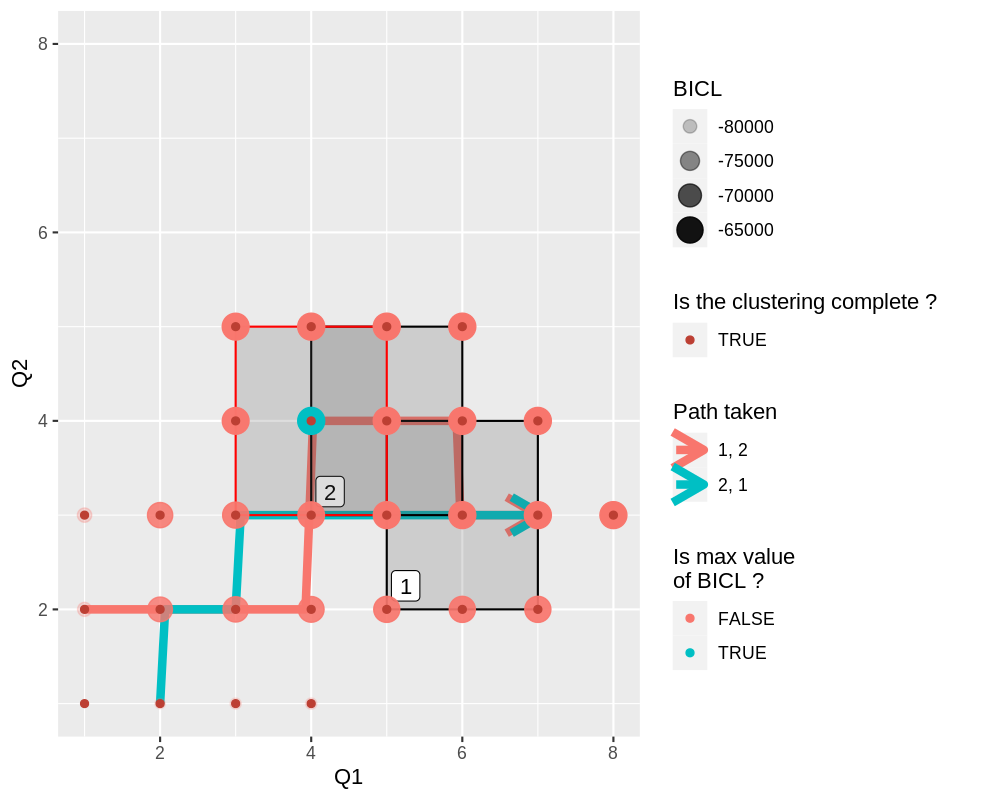
\includegraphics[scale=0.22]{img/moving_window.png}
                \caption{Exemple de parcours de fenêtre glissante}
            \end{figure}
        \end{column}
        \begin{column}{0.4\linewidth}
            \definecolor{mypurple}{RGB}{128,0,128}
            \begin{tikzpicture}

                \tikzstyle{model}=[circle,draw=none,fill=gray]
                \tikzstyle{split}=[>=stealth,->,thick, draw=blueind]
                \tikzstyle{merge}=[>=stealth,->,thick, draw=red]
                \draw[step=1cm, help lines] (-2,-2) grid (2,2);
                \node[model] (mode) at (0,0) {{\color{red}X}};

                \onslide<2->{
                    \draw[color=red, line width=1pt] (-1.5,-1.5) rectangle ++(3,3);
                }
                \onslide<3-3>{
                    \node[model] (bottom_left) at (-1,-1) {};
                    \node[model, opacity=0.6] (row_1) at (0,-1) {};
                    \node[model, opacity=0.6] (col_1) at (-1,0) {};

                    \draw[split] (bottom_left) -- (col_1);
                    \draw[split] (-1.75,0) -- (col_1);
                    \draw[split] (bottom_left) -- (row_1);
                    \draw[split] (0,-1.75) -- (row_1);
                }
                \onslide<4->{
                    \node[model] (bottom_left) at (-1,-1) {};
                    \node[model, draw=blue] (row_1) at (0,-1) {};
                    \node[model, draw=blue] (col_1) at (-1,0) {};
                }
                \onslide<4-4>{
                    \node[model, opacity=0.6] (row_2) at (1,-1) {};
                    \node[model, opacity=0.6] (col_2) at (-1,1) {};

                    \draw[split] (col_1) -- (col_2);
                    \draw[split] (-1.75,1) -- (col_2);
                    \draw[split] (row_1) -- (row_2);
                    \draw[split] (1,-1.75) -- (row_2);
                    \draw[split] (row_1) -- (mode);
                    \draw[split] (col_1) -- (mode);
                }
                \onslide<5->{
                    \node[model, draw=blue] (row_2) at (1,-1) {};
                    \node[model, draw=blue] (col_2) at (-1,1) {};
                    \node[model, draw=blue] (mode) at (0,0) {{\color{red}X}};
                }
                \onslide<5-5>{
                    \node[model, opacity=0.6] (row_3) at (1,0) {};
                    \node[model, opacity=0.6] (col_3) at (0,1) {};

                    \draw[split] (col_2) -- (col_3);
                    \draw[split] (row_2) -- (row_3);
                    \draw[split] (mode) -- (row_3);
                    \draw[split] (mode) -- (col_3);
                }
                \onslide<6->{
                    \node[model, draw=blue] (row_3) at (1,0) {};
                    \node[model, draw=blue] (col_3) at (0,1) {};
                }
                \onslide<6-6>{
                    \node[model, opacity=0.6] (top_right) at (1,1) {};
                    \draw[split] (col_3) -- (top_right);
                    \draw[split] (row_3) -- (top_right);
                }
                \onslide<7->{
                    \node[model, draw=blue] (top_right) at (1,1) {};
                }
                \onslide<8->{
                    \node[model, draw=mypurple] (top_right) at (1,1) {};
                    \node[model, draw=mypurple] (row_3) at (1,0) {};
                    \node[model, draw=mypurple] (col_3) at (0,1) {};
                    \node[model, draw=mypurple] (row_2) at (1,-1) {};
                    \node[model, draw=mypurple] (col_2) at (-1,1) {};
                    \node[model, draw=mypurple] (mode) at (0,0) {{\color{red}X}};
                    \node[model, draw=red] (bottom_left) at (-1,-1) {};
                    \node[model, draw=mypurple] (row_1) at (0,-1) {};
                    \node[model, draw=mypurple] (col_1) at (-1,0) {};

                    \draw[merge] (1,1.75) -- (top_right);
                    \draw[merge] (1.75,1) -- (top_right);
                    \draw[merge] (0,1.75) -- (col_3);
                    \draw[merge] (1.75,0) -- (row_3);
                    \draw[merge] (1.75,-1) -- (row_2);
                    \draw[merge] (-1,1.75) -- (col_2);

                    \draw[merge] (top_right) -- (col_3);
                    \draw[merge] (top_right) -- (row_3);
                    \draw[merge] (col_3) -- (col_2);
                    \draw[merge] (row_3) -- (row_2) ;
                    \draw[merge] (row_3) -- (mode);
                    \draw[merge] (col_3) -- (mode);
                    \draw[merge] (col_2) --(col_1);
                    \draw[merge] (row_2) -- (row_1);
                    \draw[merge] (mode) -- (row_1);
                    \draw[merge] (mode) -- (col_1);
                    \draw[merge] (col_1) -- (bottom_left);
                    \draw[merge] (row_1) -- (bottom_left);
                }
            \end{tikzpicture}
        \end{column}
    \end{columns}
\end{frame}

\begin{frame}
    \frametitle{Clustering de réseaux}
    \begin{columns}
        \begin{column}{0.2\linewidth}
            \begin{block}{Objectif}
                Déterminer une partition qui maximise la somme du BICL de ses sous-collections.
            \end{block}
        \end{column}
        \begin{column}{0.78\linewidth}
            \begin{tikzpicture}
                \tikzstyle{instruct}=[font=\small, text justified, rectangle,draw,fill=yellow!50]
                \tikzstyle{first_col}=[rectangle, text justified, draw,fill=gray!50]
                \tikzstyle{second_col}=[scale=0.55, circle, draw,fill=red!50]
                \tikzstyle{test}=[font=\small, text justified, diamond, aspect=2.5,thick,
                draw=blue,fill=yellow!50,text=blue]
                \tikzstyle{es}=[font=\small, text justified, rectangle,draw,rounded corners=4pt,fill=cyanind!25]

                \node[es] (liste) at (0,4) {Donner une collection à partitionner};
                \node[instruct, text width=5cm, below = 0.45cm of liste] (1-collection) {Ajuster \emph{colBiSBM}};
                \node[first_col, right = 0.5cm of 1-collection] (1-col-obj) {};
                \node[instruct, text width=5cm, below = 0.45cm of 1-collection] (dissimi) {Calculer une matrice de dissimilarité de la collection};
                \node[instruct, text width=5cm, below = 0.45cm of dissimi] (2-sous-collection) {Séparer la \emph{collection en 2 sous-collections} et ajuster les \emph{colBiSBM}};
                \node[second_col, right = 0.25cm of 2-sous-collection] (1-sec-col-obj) {1};
                \node[second_col, right = 0.25cm of 1-sec-col-obj] (1-sec-col-obj) {2};
                \node[test,below = 0.45cm of 2-sous-collection, scale=0.5] (BICL-test) {$\sum_{i=1}^{2} (\text{BIC-L}(\tikz[baseline=-0.25cm]{\node[second_col] {i};} )) > \text{BIC-L}(\tikz[baseline=-0.25cm]{\node[first_col] {};})$?};
                \node[es, right = 0.55cm of BICL-test] (sortie) {Renvoyer \tikz{\node[rectangle, draw, fill=gray!50, rounded corners=0pt] {};}};
                \node[es, left = 0.45cm of dissimi, text width = 2cm] (recursion) {Recommencer sur \tikz{\node[second_col] {1};} et \tikz{\node[second_col] {2};} };

                \tikzstyle{suite}=[->,>=stealth,thick,rounded corners=4pt]
                \draw[suite] (liste) -- (1-collection);
                \draw[suite] (1-collection) -- (dissimi);
                \draw[suite] (dissimi) -- (2-sous-collection);
                \draw[suite] (2-sous-collection) -- (BICL-test);
                \draw[suite] (BICL-test) -| node[near start, above, fill=none] {Oui} (recursion);
                \draw[suite] (recursion.north) |- (1-collection.west);
                \draw[suite] (BICL-test) -- node[near start, above, fill=none] {Non} (sortie);

            \end{tikzpicture}
        \end{column}
    \end{columns}
    \blfootnote{Même approche que~\cite{chabert-liddellLearningCommonStructures2023}}
\end{frame}

\section{Application}
\label{sec:application}
\begin{frame}
    \frametitle{Application, données plantes pollinisateurs}
    \small
    Voici des résultats du modèle \emph{iid-colBiSBM} sur des données
    plantes-pollinisateurs (~\cite{doreRelativeEffectsAnthropogenic2021}
    et~\cite{thebaultDatabasePlantpollinatorNetworks2020})
    % DONE Ajouter un tableau avec le nombre de réseaux dans chaque sous-collection
    \begin{columns}
        \begin{column}{0.48\linewidth}
            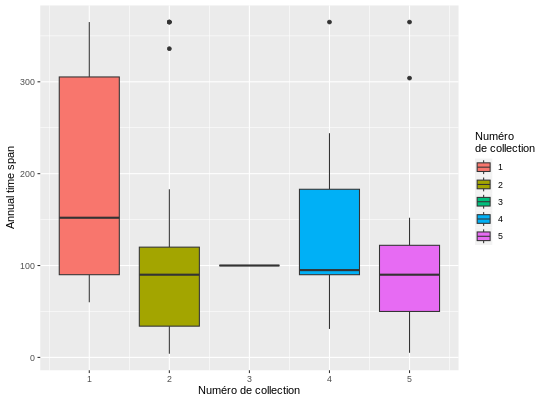
\includegraphics[scale=0.32]{img/annual_time_span_vs_iid.png}
            \begin{center}
                \begin{tabular}{ |c|c|c|c|c|c| }
                    \hline
                    \thead{N° de     \\collection} & 1 & 2 & 3 & 4 & 5 \\
                    \hline
                    \thead{Nombre de \\réseaux} & 38 & 45 & 1 & 20 & 19 \\
                    \hline
                \end{tabular}
            \end{center}
        \end{column}
        \begin{column}{0.48\linewidth}
            \begin{figure}[H]
                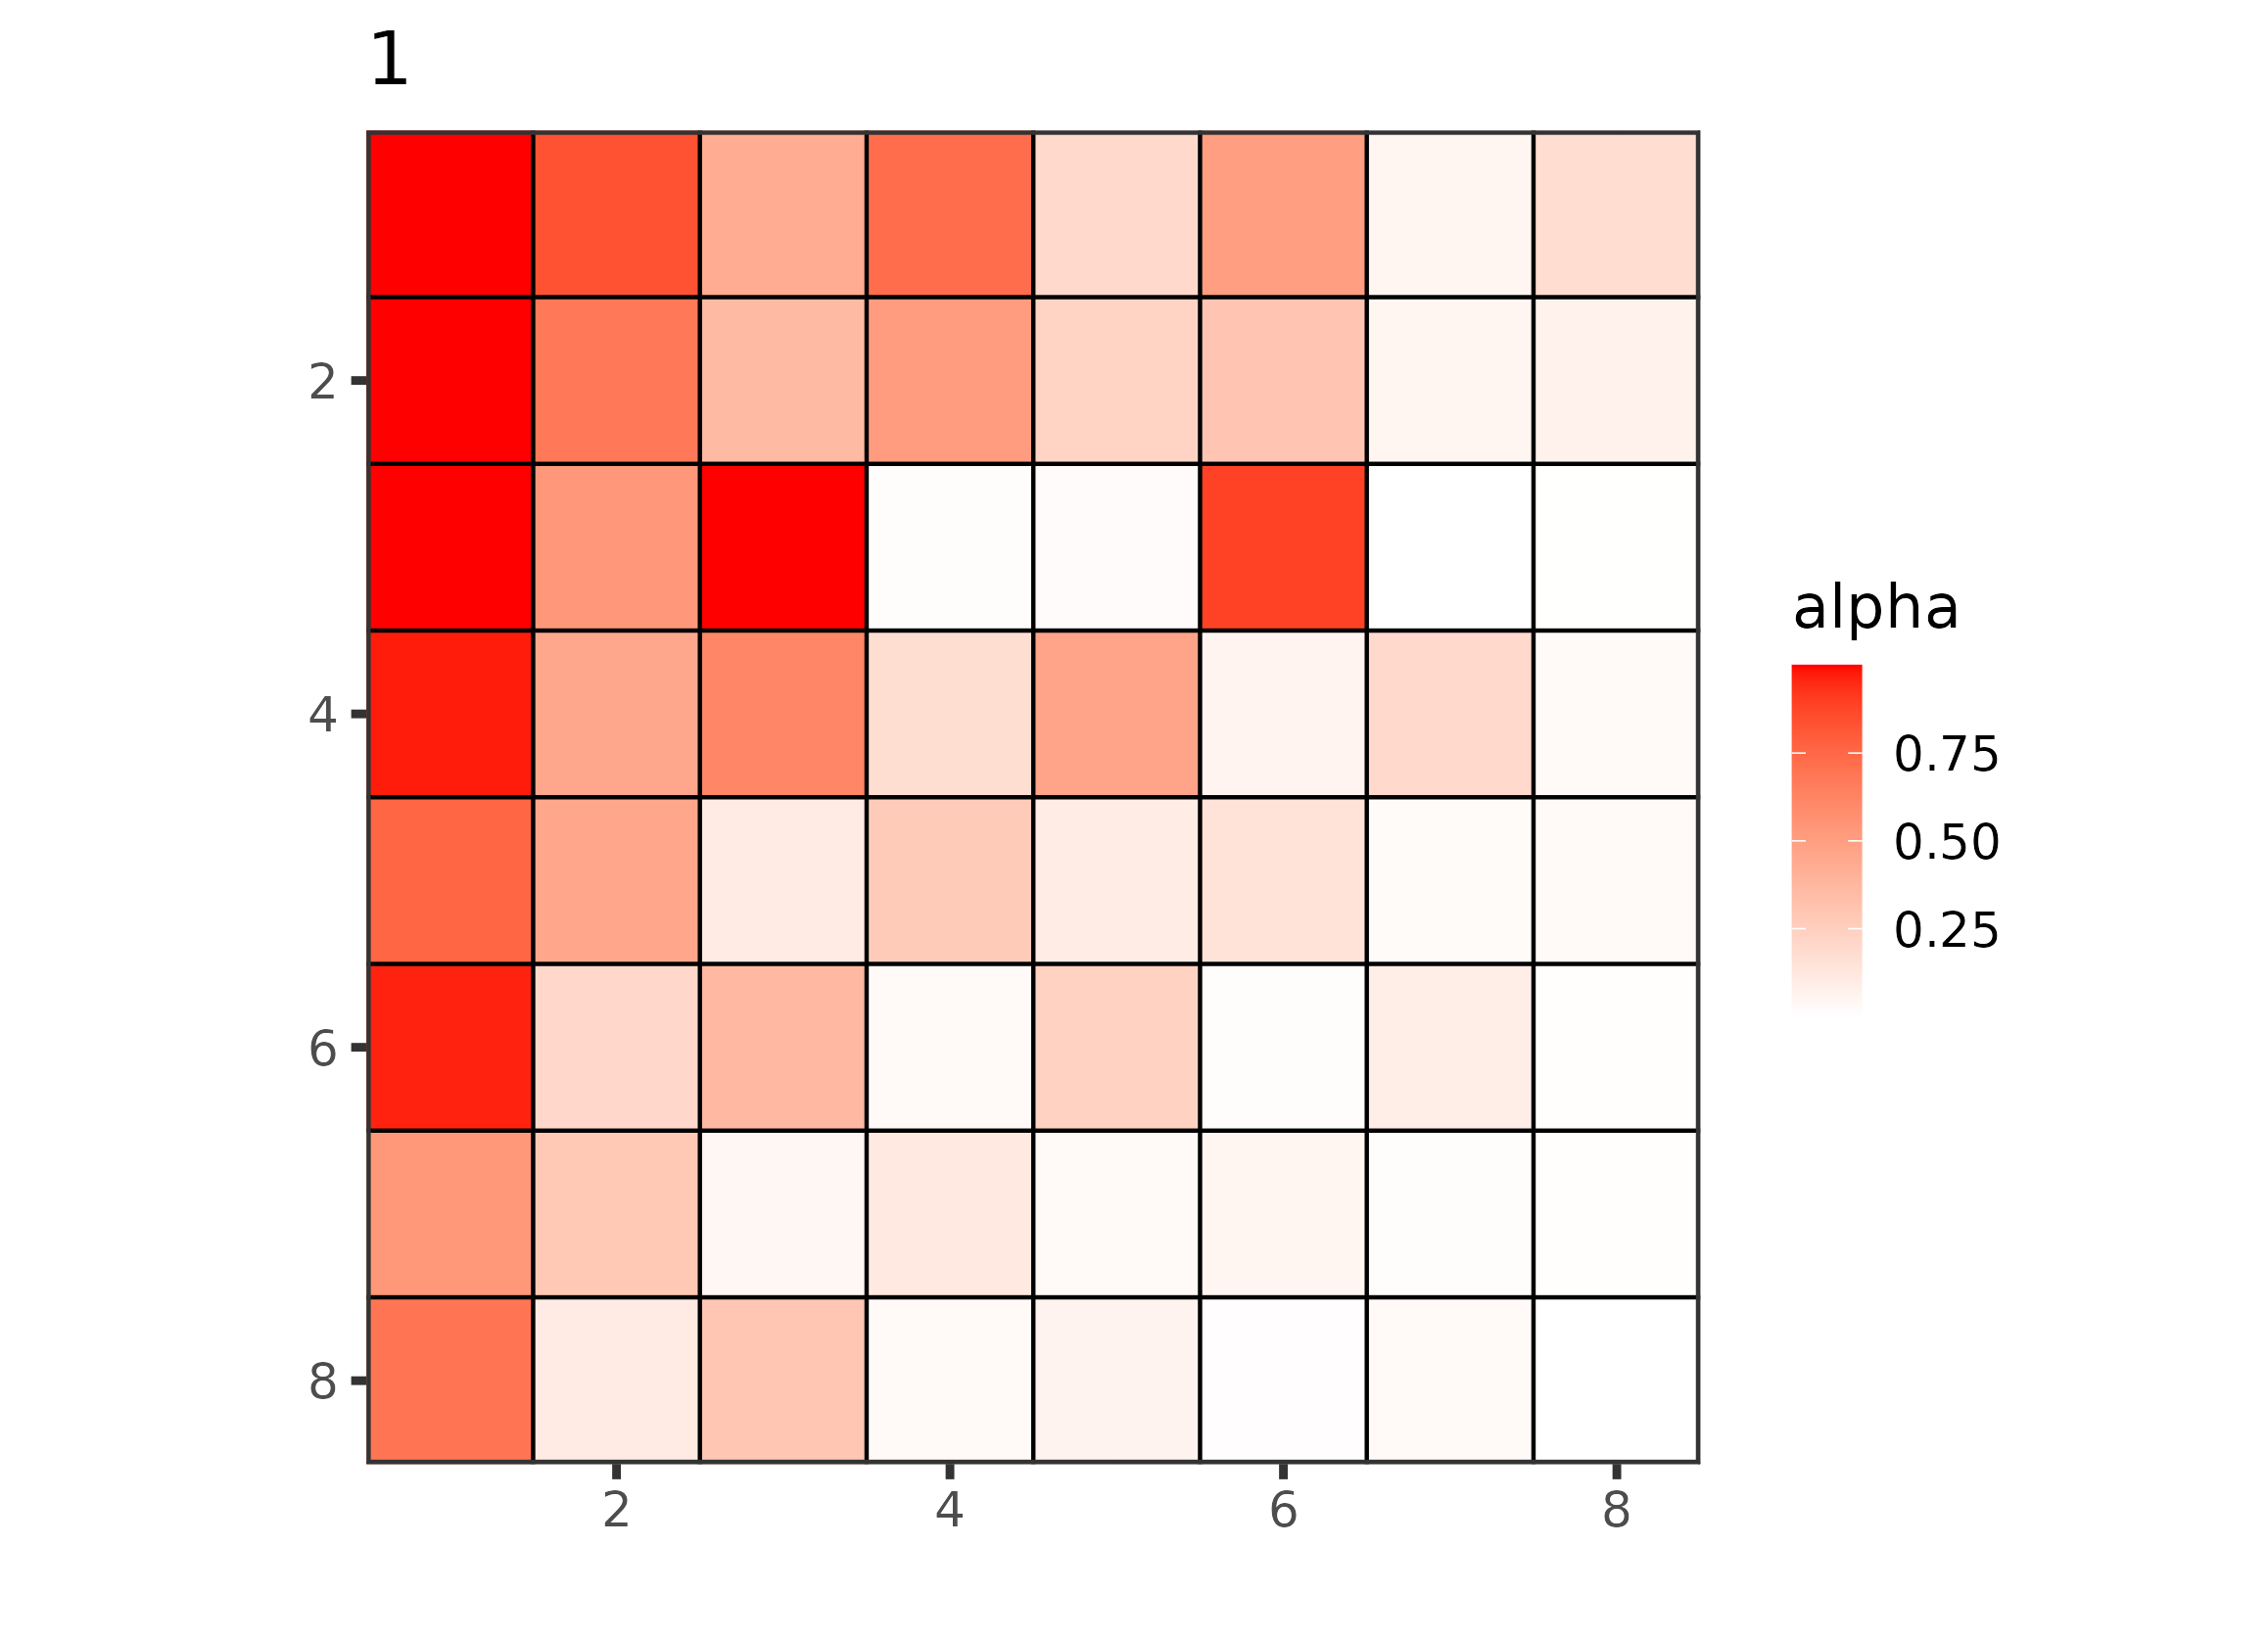
\includegraphics[width=0.45\textwidth]{img/iid-meso-1.png}
                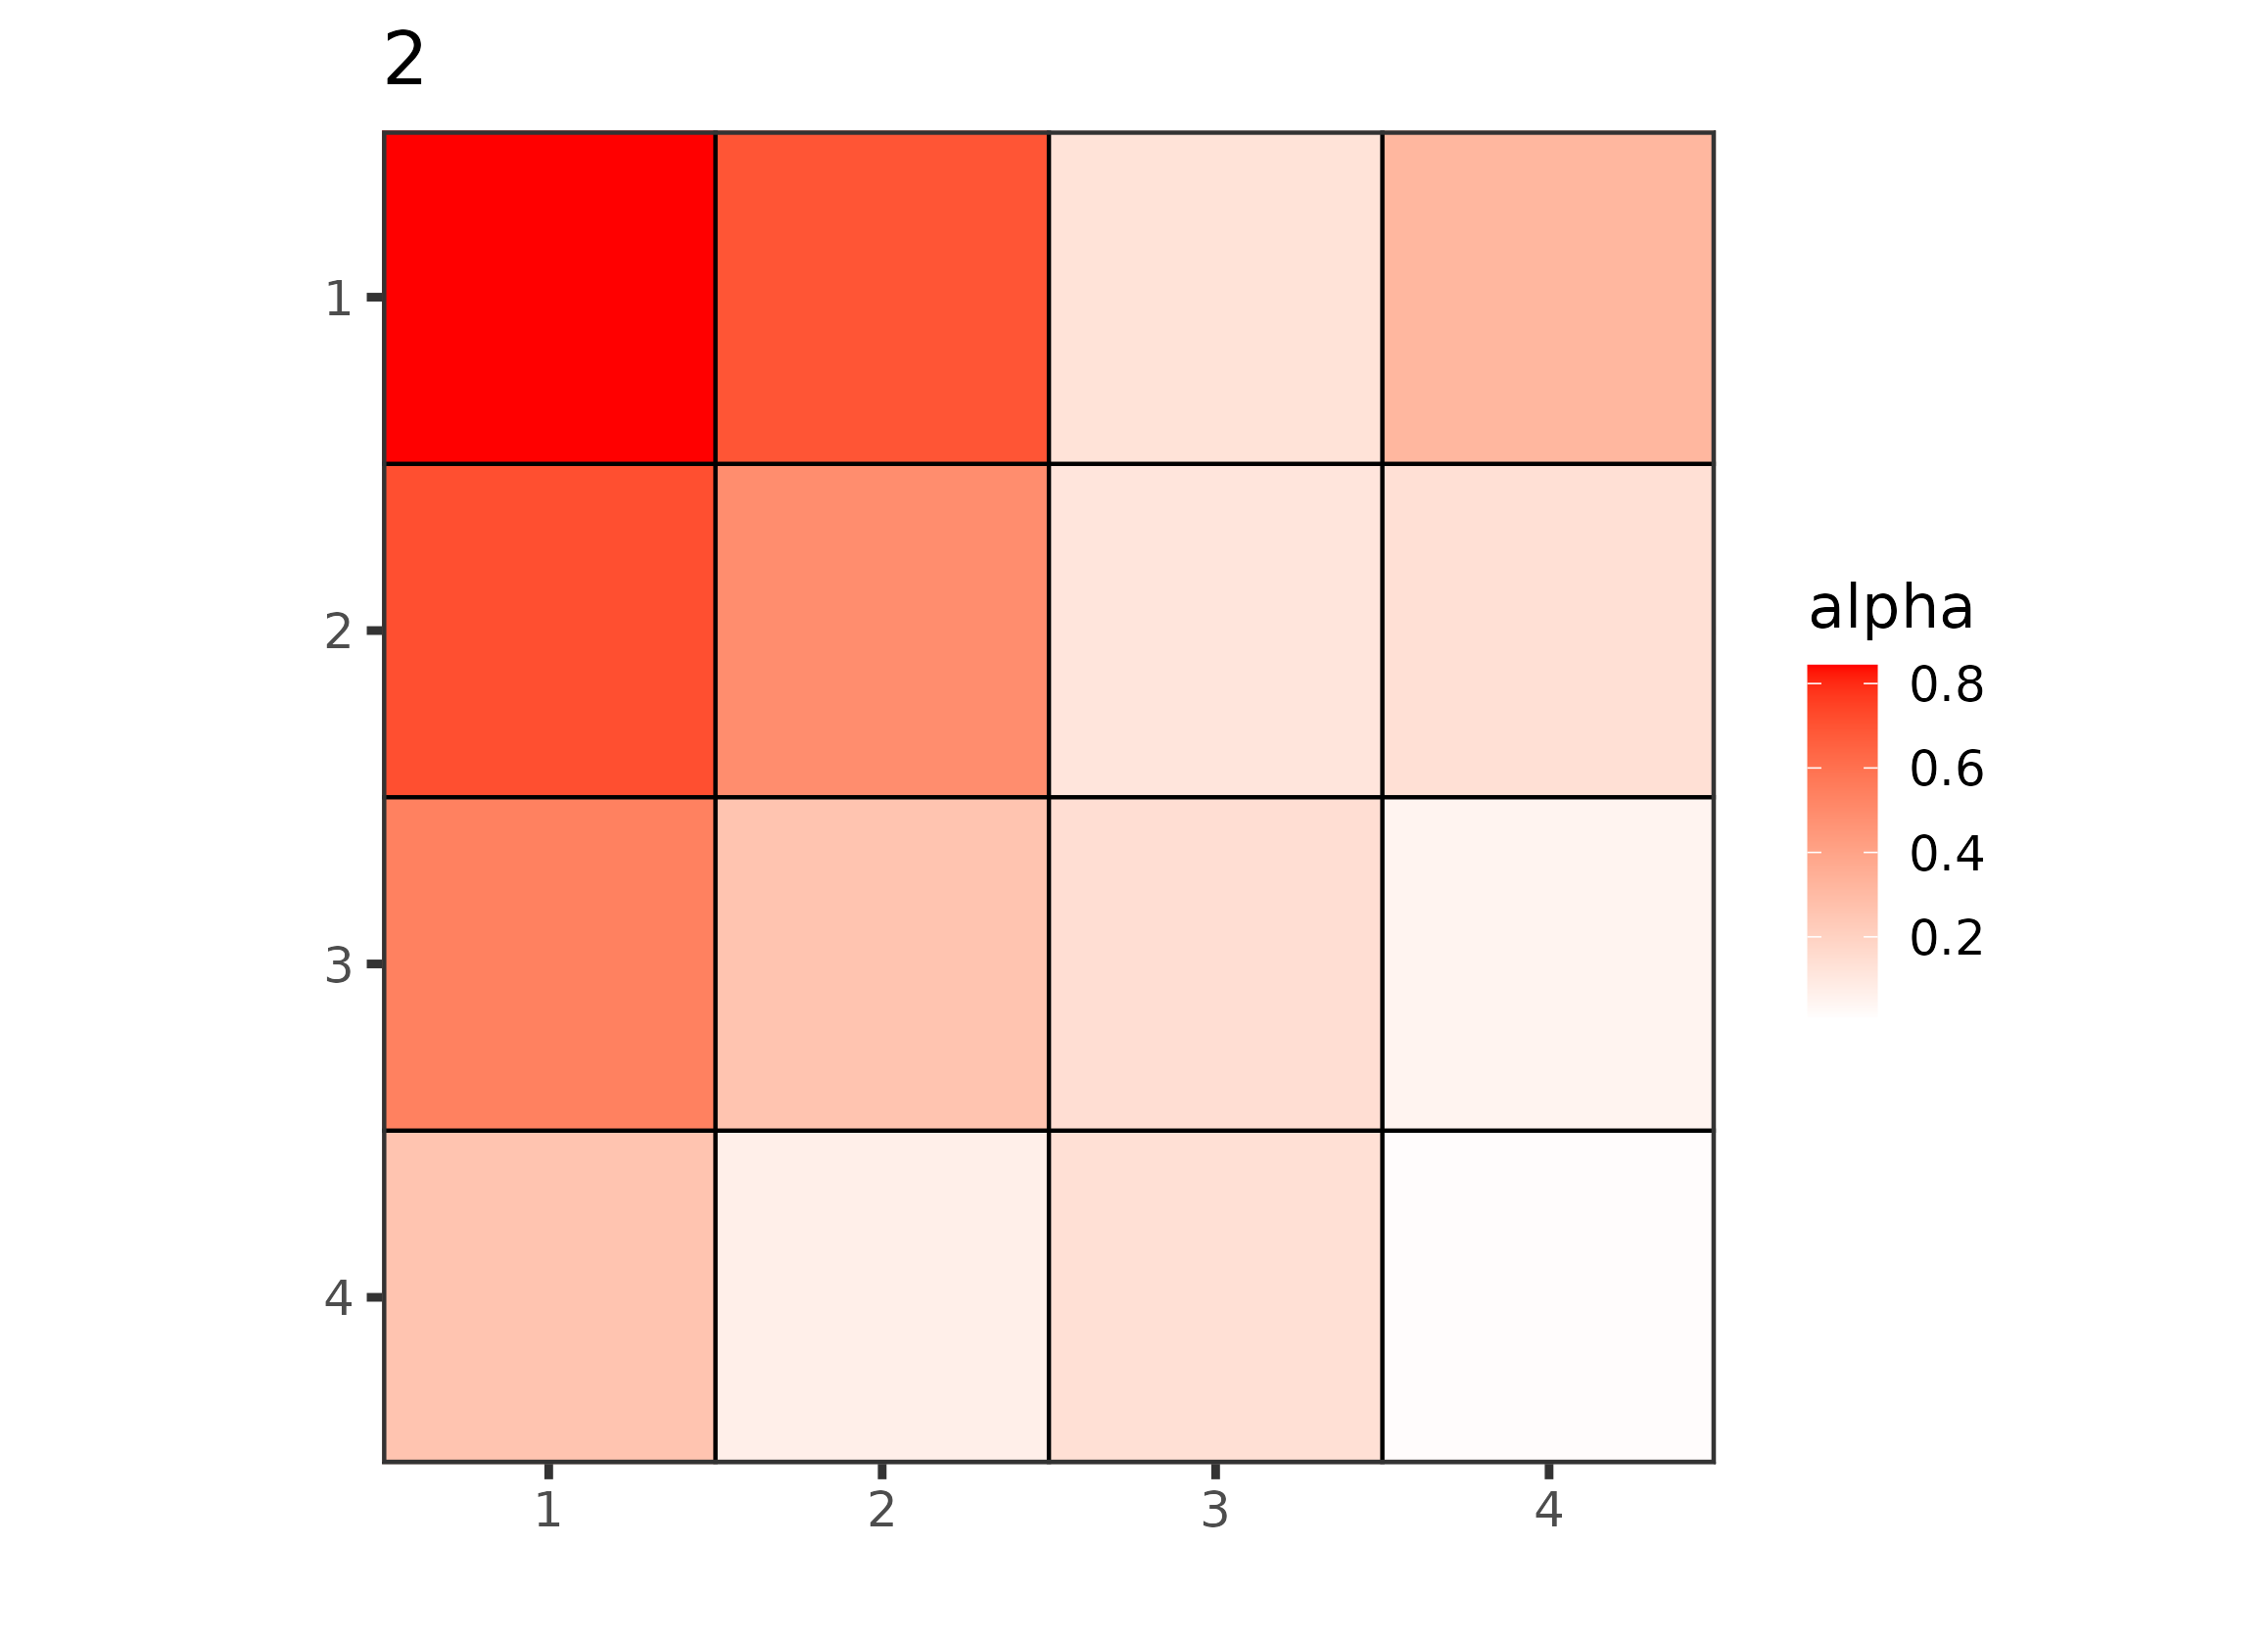
\includegraphics[width=0.45\textwidth]{img/iid-meso-2.png}
                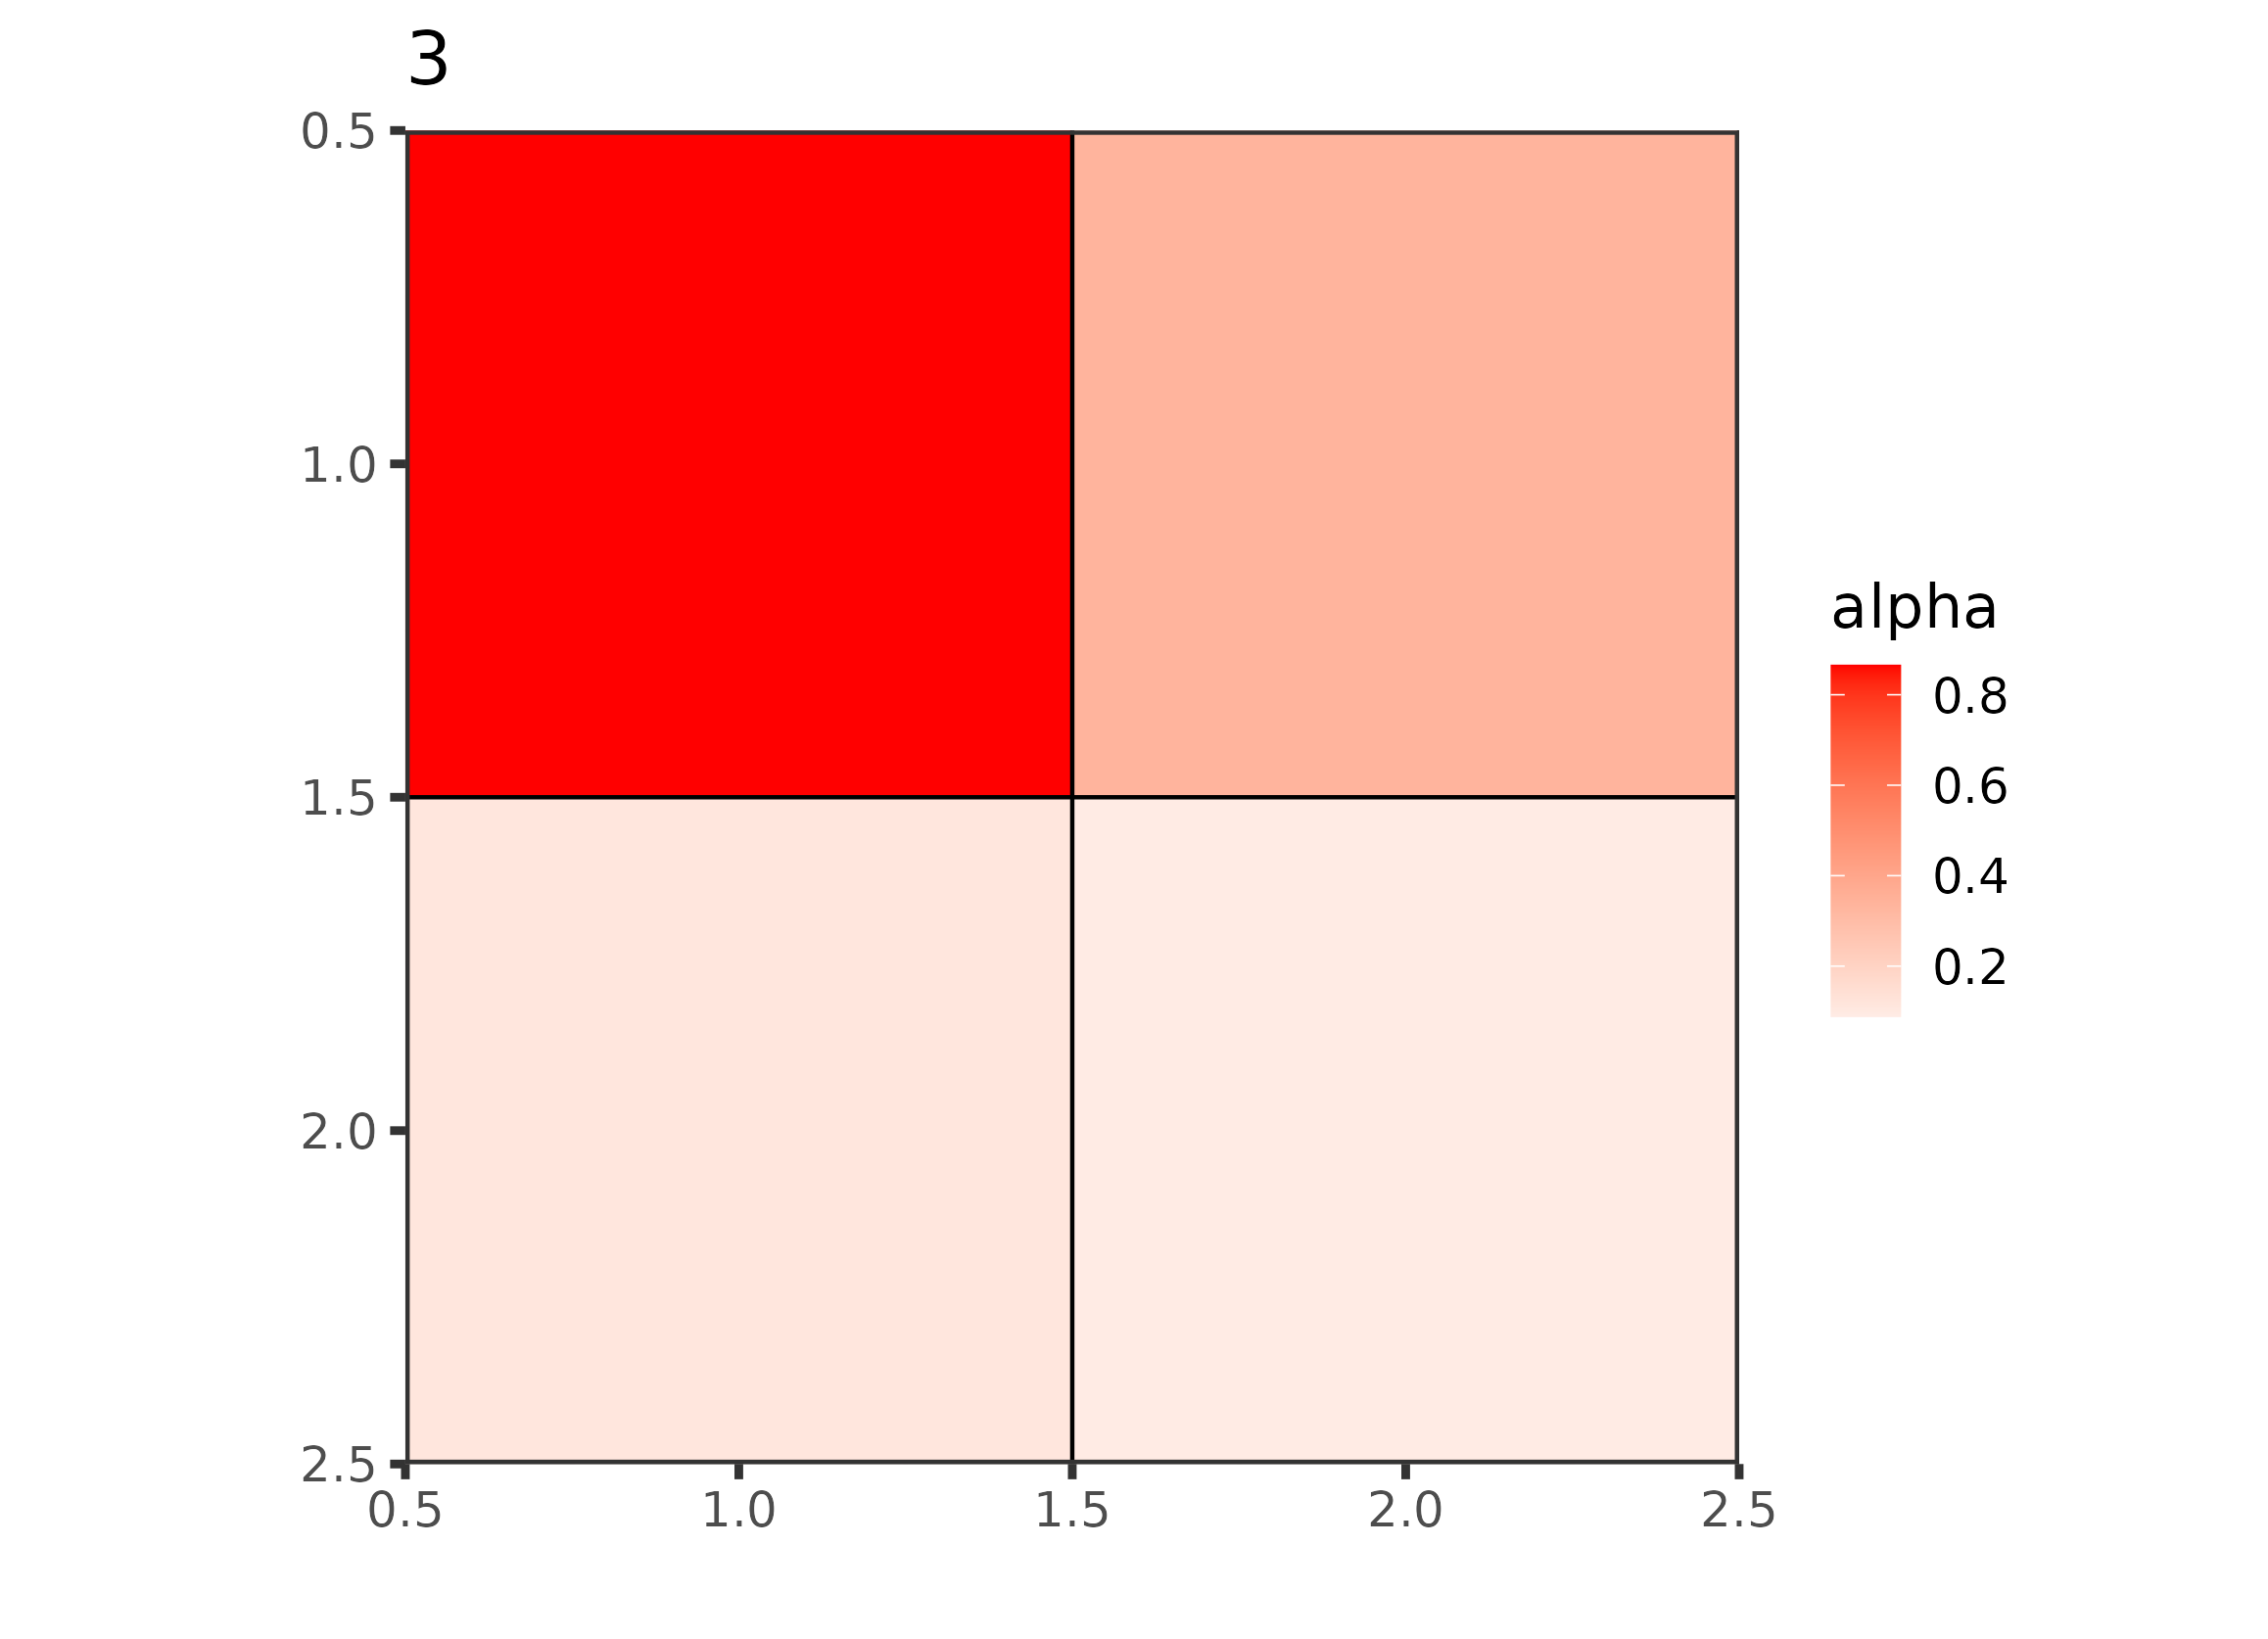
\includegraphics[width=0.45\textwidth]{img/iid-meso-3.png}
                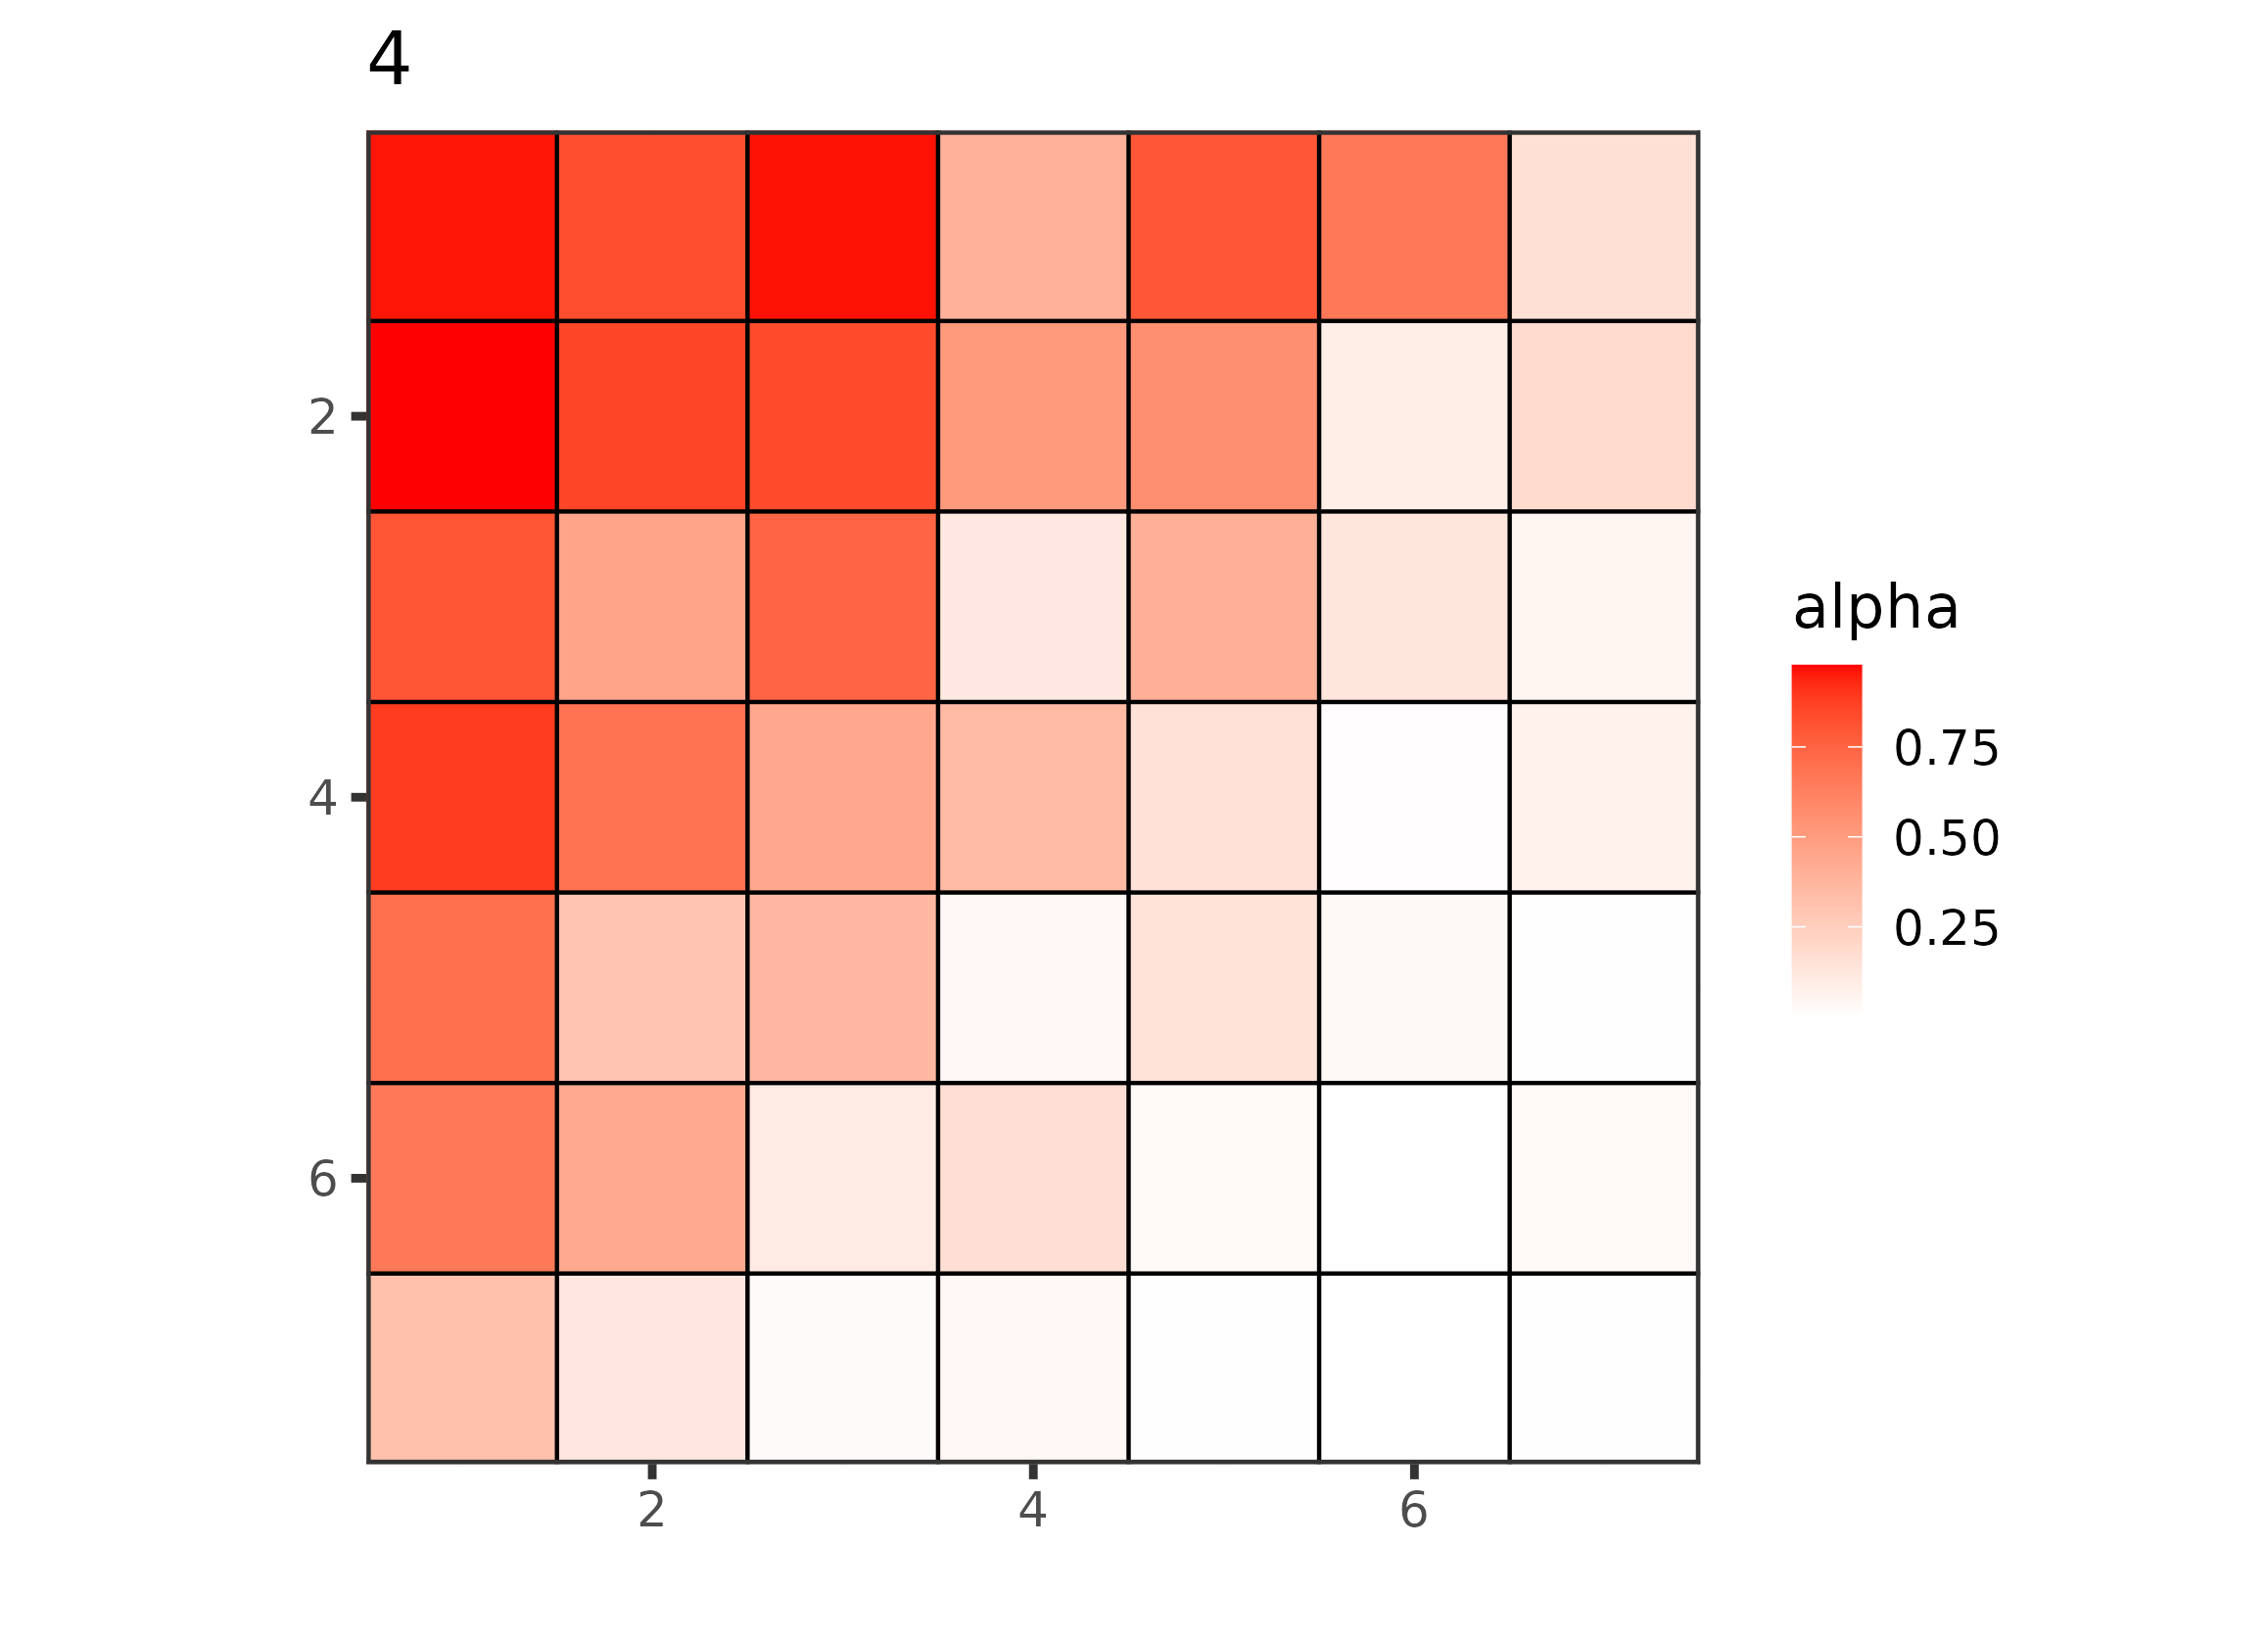
\includegraphics[width=0.45\textwidth]{img/iid-meso-4.png}
                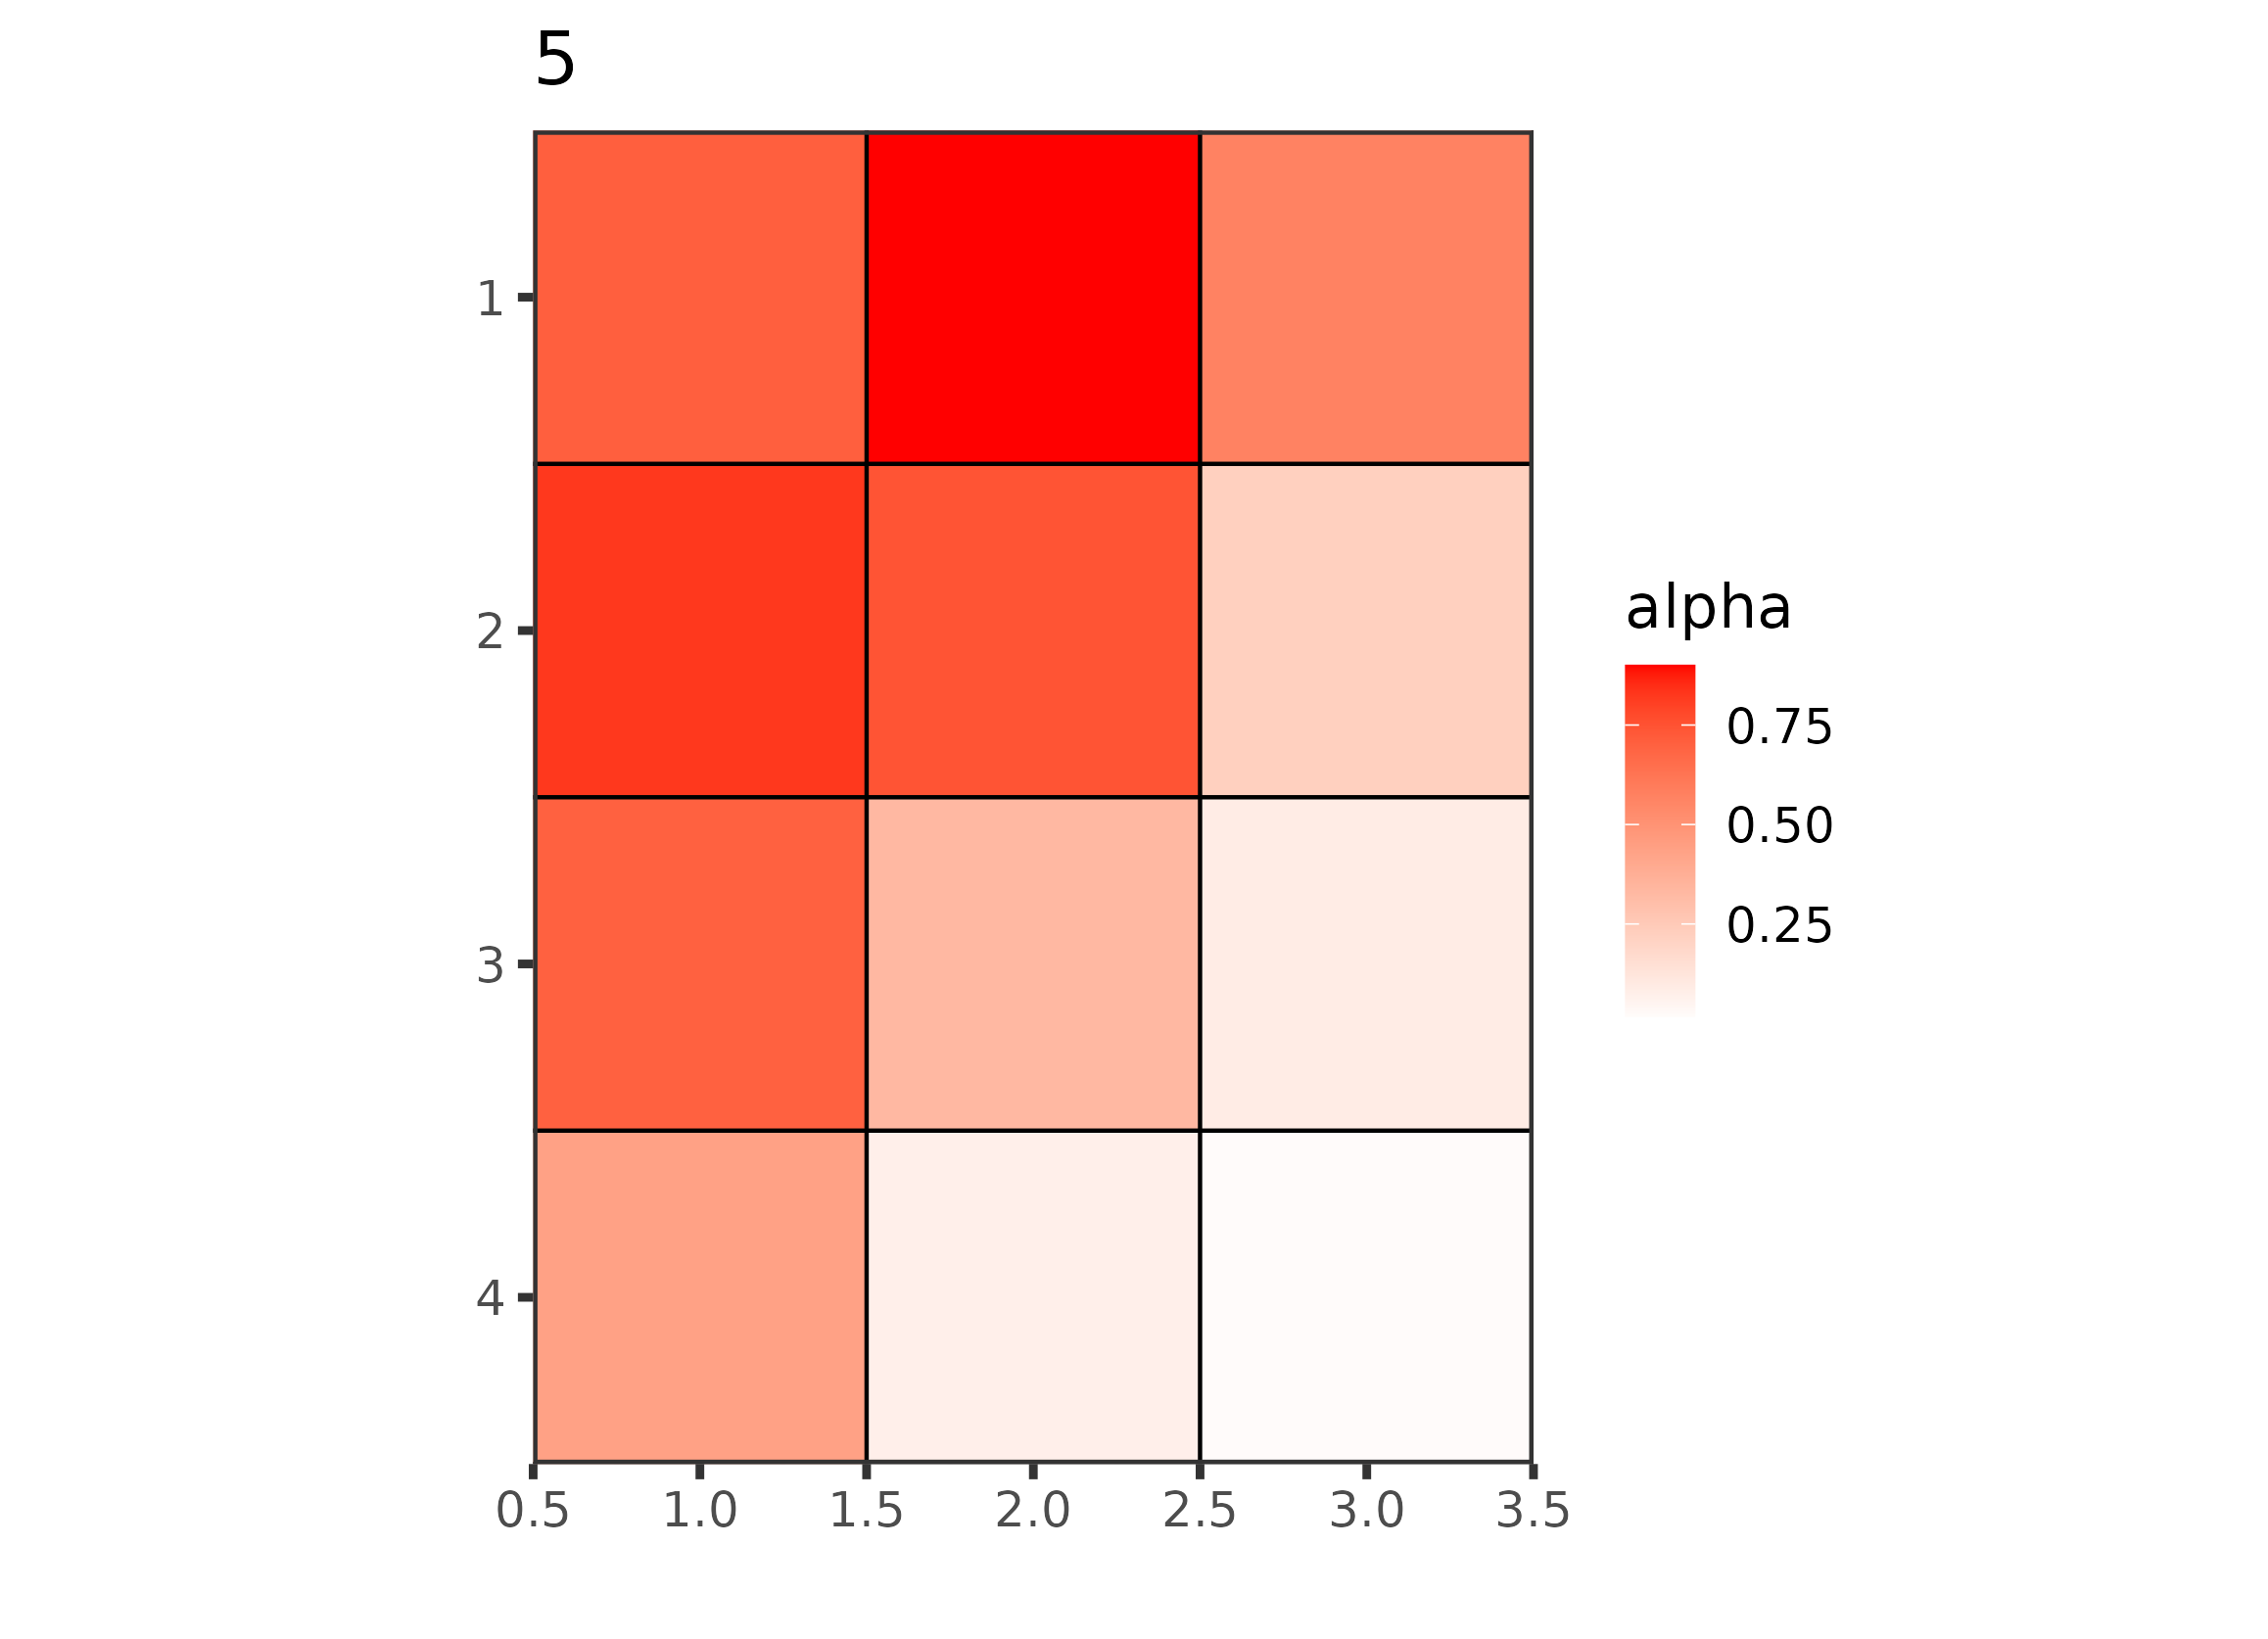
\includegraphics[width=0.45\textwidth]{img/iid-meso-5.png}
                \caption{Connectivités de la partition}
            \end{figure}
        \end{column}
    \end{columns}
\end{frame}
\section{Conclusion}
\label{sec:conclusion}
\begin{frame}
    \frametitle{Conclusion et perspectives}
    % DONE Ajouter une slide conclusion perspective
    % Rappeler les modeles avec clustering
    % Evoquer l'analyse de reseaux corrigés pour l'échantillonnage
    % Lien vers le package

    \begin{itemize}
        \item 4 modèles dont 3 qui ont une flexibilité sur au moins une des dimensions (adaptabilité aux données)
        \item Partitionner un ensemble de réseaux selon leurs structures
        \item Comparer les \emph{clusterings} de réseaux obtenus entre données brutes et données corrigées (par exemple par la méthode \emph{CoOPLBM}\footnote{~\cite{anakokDisentanglingStructureEcological2022}})
    \end{itemize}

    \bigskip
    \centering
    Le package est disponible sur GitHub : \faGithub  \url{https://github.com/Chabert-Liddell/colSBM}

    \bigskip
    \huge
    Merci pour votre attention !

\end{frame}
\renewcommand{\pgfuseimage}[1]{\scalebox{.75}{\includegraphics{#1}}}
\begin{frame}[noframenumbering,plain,allowframebreaks]
    \frametitle{Bibliographie}
    \printbibliography
\end{frame}

\end{document}